\chapter{Subcellular Localisation of Nascent IFIT Proteins in the Context of RSV Inclusion Bodies} \label{ch:Subcellular Localisation of Nascent IFIT Proteins in the Context of RSV Inclusion Bodies}
\section{Background and Aims} \label{sec:Background and Aims-Chapter3}









As established in the previous chapters, human \textit{IFIT} genes are induced following human and bovine RSV infections and thus have the propensity to enforce their anti-RSV role \textit{in vivo}. On the other hand, bovine \textit{IFITs} responses to human and bovine RSV infections were limited, however this could be due to potential higher basal expression of these genes. Drori et al. reported ectopicaly expressed human IFIT1, IFIT2, and IFIT3 to inhibit the growth of hRSV, however the mechanism of action remains to be elucitated \cite{Drori2020InfluenzaProteins}. IFIT proteins have been reported to enact their antiviral functions via multitude of mechanisms, which range between the different IFIT proteins. These range from direct interactions of IFIT1 and IFIT5 with 5'-RNA modifications \cite{Abbas2013StructuralProteins, Diamond2014IFIT1:Translation}, IFIT2 pro-apoptotic action, which is mediated via direct interactions with mitochondrial membranes \cite{Chen2017InhibitionApoptosis}, and IFIT3 mediated RIG-I signalling poentiation through the formation a scaffold between MAVS and TBK1 on mitochondrial membranes \cite{Liu2011IFN-InducedTBK1}. IFIT1, IFIT2, and IFIT3 have also been observed to form heterodimer and heterotrimer protein complexes, which increase the IFIT stability and can influence the functions of these proteins \cite{Mears2018BetterResponse}. Assesing the subcellular localisation of IFIT protiens in infected cells could therefore act as a proxy for their RSV inhibitory mechanism of action. We hypothetise that the sites of IFIT/RSV interactions are the RSV inclusion bodies. These structures ...




We hypothetise ... first look at localisation to gauge potential mechanisms of interactions ... the inhibition could be IB mediated ... what are ibs ... 




Intro about RSV IB, its components, function and known siphoning about increasing size increasing maturity





First aim: look at how does cellular and subcellular localisation changes in response to infection, which could suggest ivolvement of IFITs with RSV lifecycle
Second aim: detaily asses the interaction of IFITs and RSV IBs during infection






\section{Results} \label{sec:Results-Chapter3}
\subsection{IFIT Subcellular Localisation During Interferon Induction and RSV Infection} \label{subsec:IFIT Subcellular Localisation During Interferon Induction and RSV Infection}
% introduction to ib stuff from my study
write about ib size statistics from my analysis

\begin{figure}
    \centering
    \includegraphics[width=1\linewidth]{08. Chapter 3/Figs/01. Localisation introduction/01. IB-zooms.pdf}
    \caption[Inclusion Bodies Within RSV Infected Cells: Zoom Sequence.]{\textbf{Inclusion Bodies Within RSV Infected Cells: Zoom Sequence.} A represerenative image of RSV infected cells detected using confocal microscopy. Cellular nuclei were stained with DAPI and are shown in yellow; RSV inclusion bodies are shown in cyan; and the cytoplasm is shown in magenta. Figure highlights a zoom sequence from a population of cells, into a single syncytia view, with lastly focusing at one individual inclusion body.}
    \label{fig:Inclusion Bodies Within RSV Infected Cells: Zoom Sequence}
\end{figure}

ibs are mainly spherical although expeptions happpen

\begin{figure}
    \begin{subfigure}{0.495\textwidth}
        \caption{}
        \includegraphics[width=\textwidth]{08. Chapter 3/Figs/01. Localisation introduction/02. heatmap_all.pdf} 
    \end{subfigure}
    \hfill
    \begin{subfigure}{0.495\textwidth}
        \caption{}
        \includegraphics[width=\textwidth]{08. Chapter 3/Figs/01. Localisation introduction/03. heatmap_a549.pdf}
    \end{subfigure}

    \medskip
    \begin{subfigure}{0.495\textwidth}
        \caption{}
        \includegraphics[width=\textwidth]{08. Chapter 3/Figs/01. Localisation introduction/04. heatmap_beas2b.pdf} 
    \end{subfigure}
    \hfill
    \begin{subfigure}{0.495\textwidth}
        \caption{}
        \includegraphics[width=\textwidth]{08. Chapter 3/Figs/01. Localisation introduction/05. heatmap_mdbk.pdf} 
    \end{subfigure}
    
    \caption[Size Characterization of Inclusion Bodies Across Different Cell Lines.]{\textbf{Size Characterization of Inclusion Bodies Across Different Cell Lines.} This figure presents the relationship between the measured area (\(\mu m^2\)) and diameter (\(\mu m\)) of individual inclusion bodies (IBs) as observed within the scope of this study. Additionally, the figure includes distinct population distributions depicted alongside the plots, representing (a) the aggregate of 1727 observations of IBs across all individual cell lines, (b) 1008 observations from the A549 cell line, (c) 99 observations from the BEAS2B cell line, and (d) 620 observations from the MDBK cell line. Contour plots are incorporated to elucidate the underlying density of individual IBs within the plots.}
    \label{fig:Size Characterization of Inclusion Bodies Across Different Cell Lines}  
\end{figure}

there is a clear difference in sizes detected in our study
compare to published and fj thesis
mdbk has more small ibs
each cell line seems to have also unusally large ibs


\begin{figure}
    \centering
    \includegraphics[width=1\linewidth]{08. Chapter 3/Figs/01. Localisation introduction/06. box-infection.pdf}
    \caption[boxplot of ib sizes per cell line.]{\textbf{boxplot of ib sizes per cell line.} this is the data from above but only area, to be able to compare it later}
    \label{fig:boxplot of ib sizes per cell line}
\end{figure}

5, 3, 2 areas



% human stuff
Asdfasfsdfasdf \newline
IF Mock | INF | Infection \newline
A549 BEAS2B

Merge pictures of clusters of cells looking at changes between subcellular localisation and a clear increase in mean intensity. Graphs show mean intensity changes from all cells imaged.

\begin{figure}
    \centering
    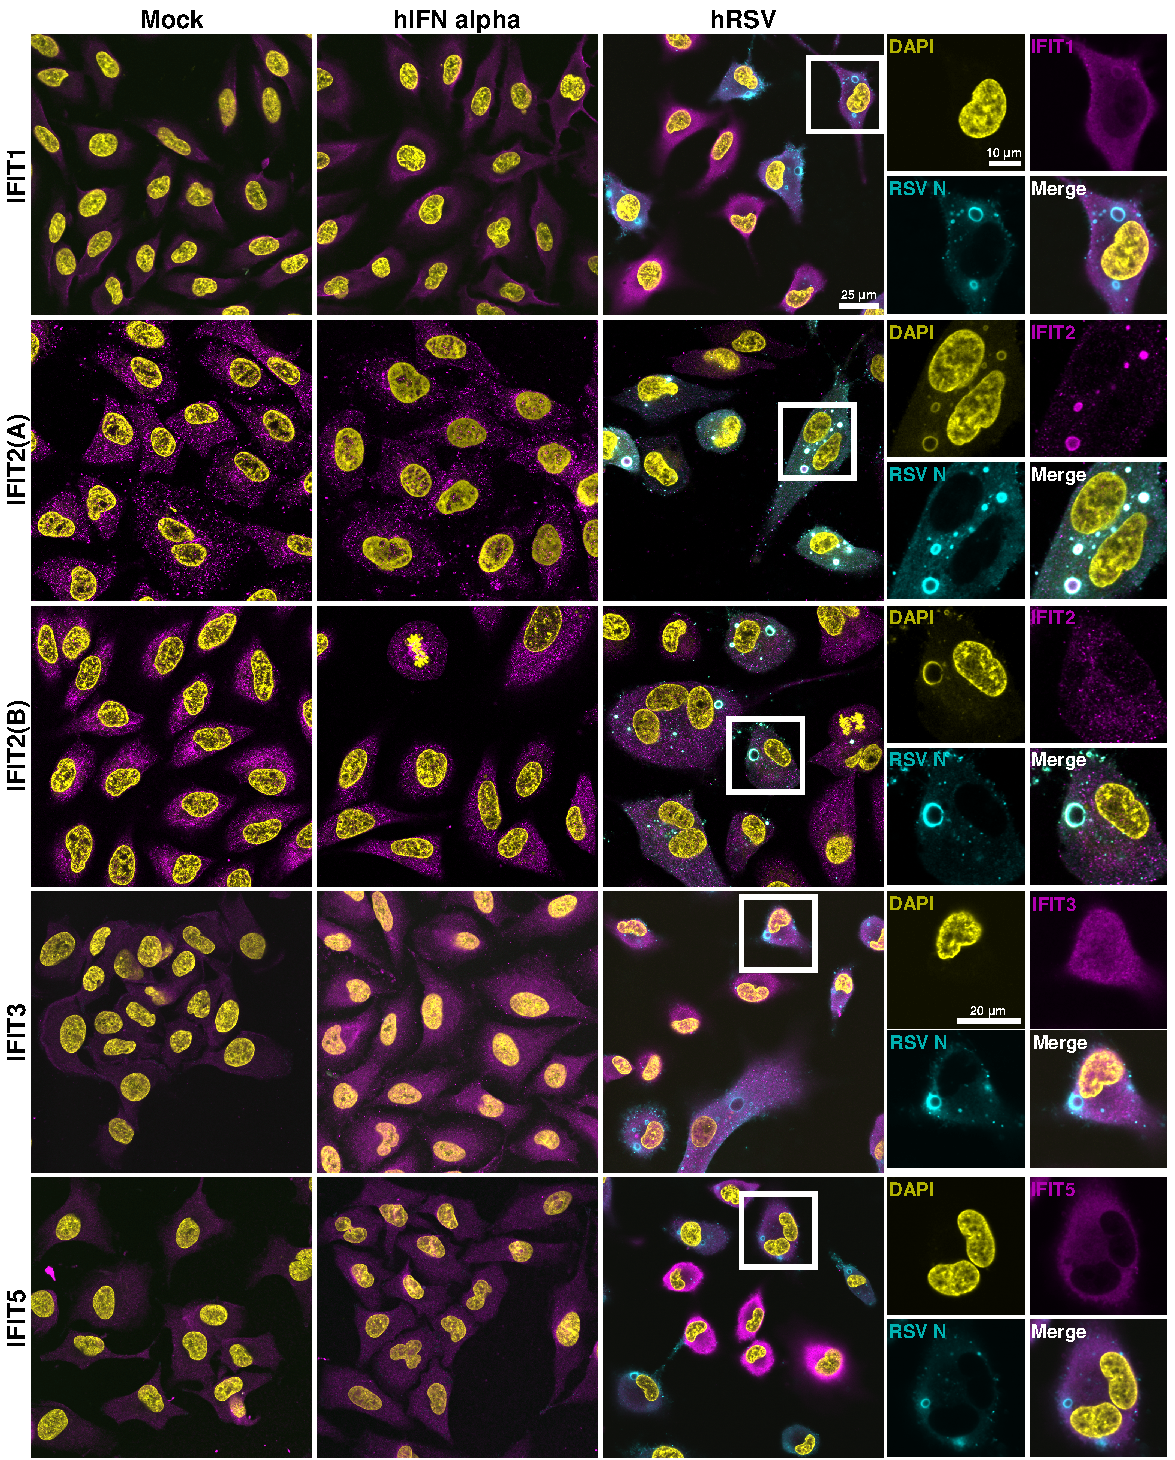
\includegraphics[width=1\linewidth]{08. Chapter 3/Figs/01. Localisation introduction/07. a549 merges.pdf}
    \caption[The Changes in Subcellular Localisation of Human IFITs in A549 Cells Subjected to hIFN\(\alpha\) or hRSV.]{\textbf{The Changes in Subcellular Localisation of Human IFITs in A549 Cells Subjected to hIFN\(\alpha\) or hRSV.} A549 cell were either mock treated, or treated with 1000 IU/mL of hIFN\(\alpha\) for 24 hours, or were infected with hRSV MOI 1 for 24 hours. Cells were fixed, and stained with DAPI (nuclei detection; yellow), anti-RSV N antibody (cyan), or with antibodies against IFIT proteins (magenta). Two antibodies against IFIT2 were used, termed IFIT2A and IFIT2B. Insets with magnified selections were created from infected images to more easily convey the underlying subcellular localisations.}
    \label{fig:The Changes in Subcellular Localisation of Human IFITs in A549 Cells Subjected to hIFNa or hRSV.}
\end{figure}

\begin{figure}
    \centering
    \includegraphics[width=1\linewidth]{08. Chapter 3/Figs/01. Localisation introduction/08. a549 plots.png}
    \caption[Quantification Of Expression Changes of Human IFITs in A549 Cells Subjected to hIFN\(\alpha\) or hRSV.]{\textbf{Quantification Of Expression Changes of Human IFITs in A549 Cells Subjected to hIFN\(\alpha\) or hRSV.} figure lened here when you finish the figure}
    \label{fig:Quantification Of Expression Changes of Human IFITs in A549 Cells Subjected to hIFNa or hRSV.}
\end{figure}


% bovine stuff
Asdfasfsdfasdf \newline
IF Mock | INF | Infection \newline
MDBK BT

Merge pictures of clusters of cells looking at changes between subcellular localisation and a clear increase in mean intensity. Graphs show mean intensity changes from all cells imaged.

\begin{figure}
    \centering
    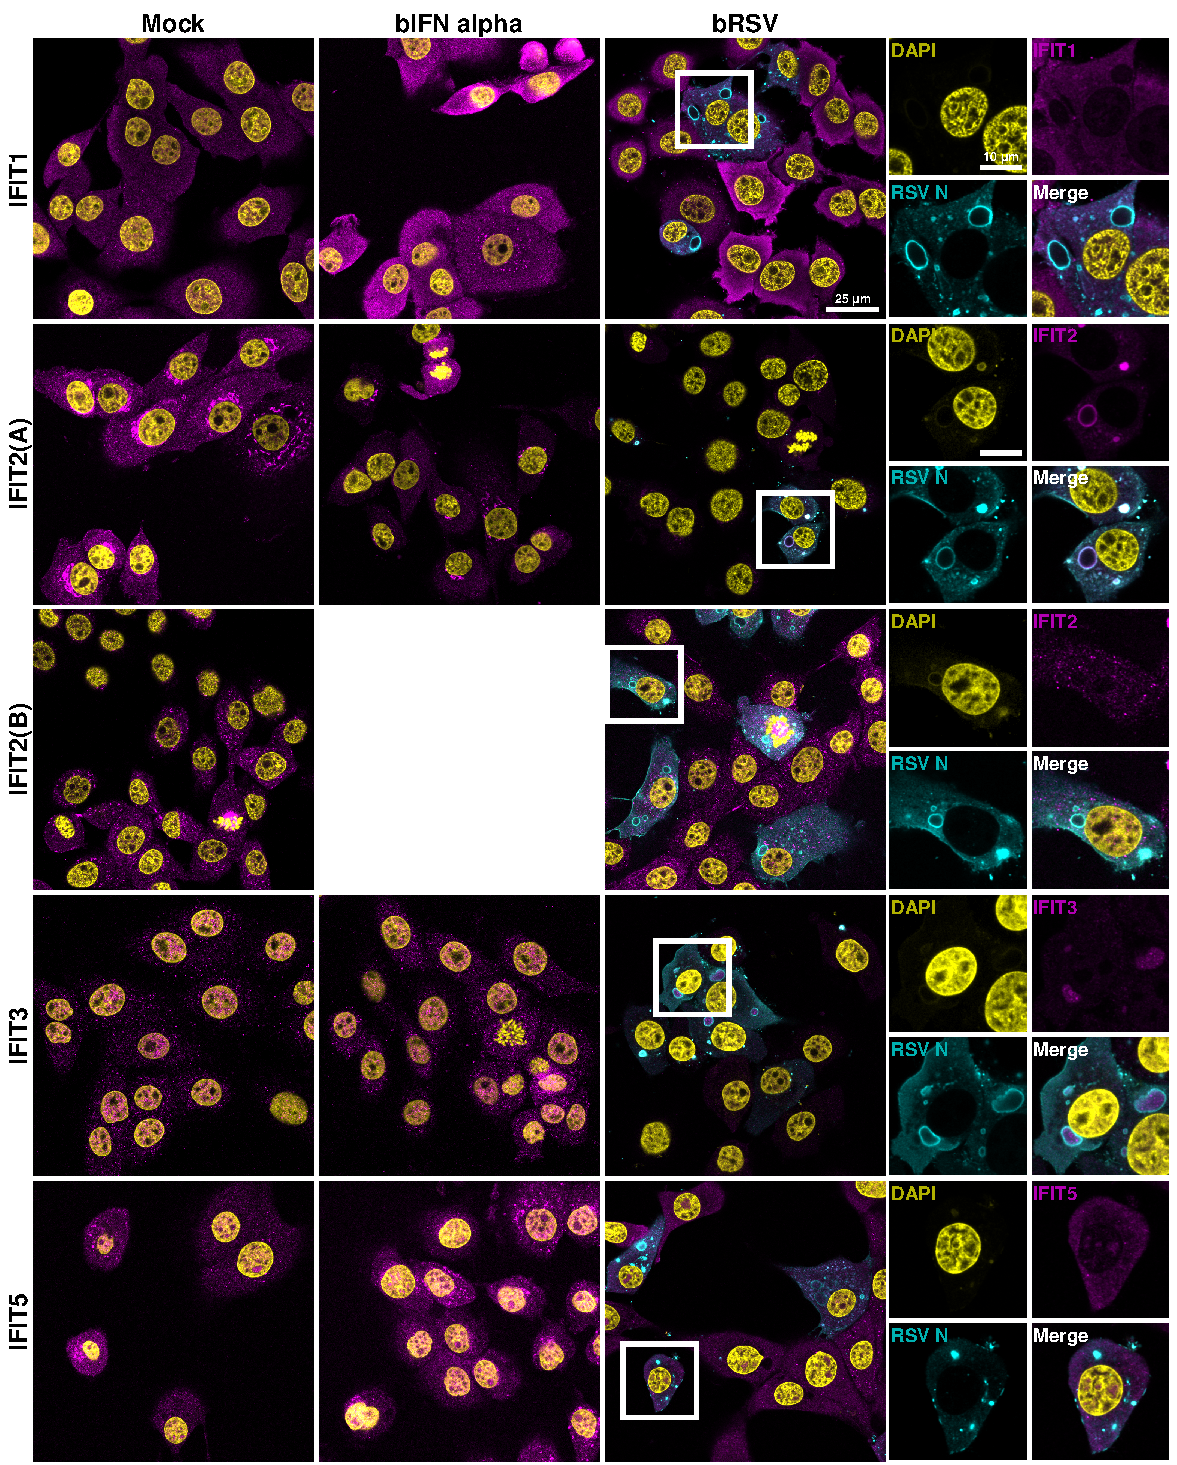
\includegraphics[width=1\linewidth]{08. Chapter 3/Figs/01. Localisation introduction/09. mdbk-merges-test.pdf}
    \caption[The Changes in Subcellular Localisation of Bovine IFITs in MDBK Cells Subjected to bIFN\(\alpha\) or bRSV.]{\textbf{The Changes in Subcellular Localisation of Bovine IFITs in MDBK Cells Subjected to bIFN\(\alpha\) or bRSV.} MDBK cell were either mock treated, or treated with 5 ng/mL of bIFN\(\alpha\) for 24 hours, or were infected with bRSV MOI 1 for 24 hours. Cells were fixed, and stained with DAPI (nuclei detection; yellow), anti-RSV N antibody (cyan), or with antibodies against IFIT proteins (magenta). Two antibodies against IFIT2 were used, termed IFIT2A and IFIT2B. Insets with magnified selections were created from infected images to more easily convey the underlying subcellular localisations.}
    \label{fig:The Changes in Subcellular Localisation of Bovine IFITs in MDBK Cells Subjected to bIFNa or bRSV}
\end{figure}

\begin{figure}
    \centering
    \includegraphics[width=1\linewidth]{08. Chapter 3/Figs/01. Localisation introduction/10. mdbk plots.png}
    \caption[Quantification Of Expression Changes of Bovine IFITs in MDBK Cells Subjected to bIFN\(\alpha\) or bRSV.]{\textbf{Quantification Of Expression Changes of Bovine IFITs in MDBK Cells Subjected to bIFN\(\alpha\) or bRSV.} figure lened here when you finish the figure}
    \label{fig:Quantification Of Expression Changes of Bovine IFITs in MDBK Cells Subjected to bIFNa or bRSV}
\end{figure}

write about the potentially interesting things we see in infection and that further detailed analysis was conducted. Describe the definitions of different phenotypes. 
\subsection{Nascent Human and Bovine IFIT Localisation During RSV Infection} \label{subsec:Nascent Human and Bovine IFIT Localisation During RSV Infection}
\subsubsection{Phenotypic Diversity of Nascent IFIT1 Interaction with RSV Inclusion Bodies}
Initial experiment suggested hIFIT1 colocalises with the hRSV IBs in A549 cell line, however assessing all 281 observation we can see that hIFIT1 displays a range of phenotypic divesity with regards to interaction with these structures. As can be seen in Figure \ref{fig:Phenotypic Diversity of hIFIT1 Interactions with hRSV Inclusion Bodies in A549 Cell Line} panel (a), 30\% of interactions result in either full or partial exclusion from the structure or an even diffusion through the IB and the surroinding cytosol. Next most common phenotype is a inclusion inside the IB structure, occuring in circa 18\% of observation. Following phenotypes, orrucing in the same frequency of 9\%, are a phenotype of colocalisation with the edge of the inclusion body joined with exclusion from the area of the IB; and a edge exclusion phenotype, where IFIT1 was present equaly between the IB and the surrounding cytoplasm with the exeption of of the IB boundry, where its signal is decreased. Representative images of the phenotypes mentioed above can be seen in Figure \ref{fig:Representative Images of Phenotypic Diversity of hIFIT1 Interactions with hRSV Inclusion Bodies in A549 Cell Line}. We have also observed IFIT1 to dysplay edge exclusion with obvoius spots within the IB structure (Edge exclusion + IBAG) and also a colocalisation with phenotype but neither had a sufficiently high frequency of occurance where we can be certain that these are indeed relevant during infection and not just imaging artefacts. In Figure \ref{fig:Phenotypic Diversity of hIFIT1 Interactions with hRSV Inclusion Bodies in A549 Cell Line} panel (b), we can observe the measured areas of the IBs associated with phenotypes which had the frequency of accurance higher than 5\%. We can see that the two most common pheotypes, exclusion and diffusion, had median IB area sizes of 5 and 4.4 \(\mu m^2\), values either identical or very similar to the aggregated median IB area of all the observations in A549 cell line. Both phenotypes also encompass a range of IB sizes, from sub 1 \(\mu m^2\) until supra 20 \(\mu m^2\) IB areas. On the other hand, the other phenotyes observed are more prevalent in larger inclusion bodies. In more detail, inclusion phenotype was more prevalent in supra 3 \(\mu m^2\) inclusion bodies, with the median size of 8; colocalisation accompanied by exclusion phenotype median IB size was 12 \(\mu m^2\), although some IBs with sizes between 0.8 to 5 \(\mu m^2\) showed this phenotype as well; and the edge exlusion phenotype was in IBs with median size of 7 \(\mu m^2\), although these IB were clustered in two clusters with median values of approximately 5 and 10 \(\mu m^2\) respectively. Our data indicates that while in majrity of cases IFIT1 is either excluded or diffused throught the IB structures, regardless ofn the IB size and thus maturity, we can see a potential interaction with more mature IBs of sizes above 5 \(\mu m^2\), which in the literature, coinsides to the IB sizes which have IBAGs present (\cite{Rincheval2017FunctionalVirus}). 

\begin{figure}
    \begin{subfigure}{0.495\textwidth}
        \caption{}
        \includegraphics[width=1\linewidth]{08. Chapter 3/Figs/02. Infection/01. IFIT1/01. bar_i1_a549.pdf} 
    \end{subfigure}
    \begin{subfigure}{0.495\textwidth}
        \caption{}
        \includegraphics[width=1\linewidth]{08. Chapter 3/Figs/02. Infection/01. IFIT1/02. box_i1_a549.pdf}
    \end{subfigure}
    \caption[Phenotypic Diversity of hIFIT1 Interactions with hRSV Inclusion Bodies in A549 Cell Line.]{\textbf{Phenotypic Diversity of hIFIT1 Interactions with hRSV Inclusion Bodies in A549 Cell Line.} A549 cells were infected with human RSV at MOI 1 and fixed 24 HPI. Cells were double-labeled with with anti-RSV N and anti-IFIT1 antibodies and imaged on confocal microscope. Panel (a) shows percentual proportions of observed phenotypes between hRSV inclusion bodies and hIFIT1 (281 observations), with the red dotted line denoting the 5\% threshold, marking phenotypes considered relevant above this limit. Panel (b) shows the IB area in \(\mu m^2\) per observed relevant phenotype.}
    \label{fig:Phenotypic Diversity of hIFIT1 Interactions with hRSV Inclusion Bodies in A549 Cell Line}
\end{figure}

\begin{figure}
    \centering
    \includegraphics[width=1\linewidth]{08. Chapter 3/Figs/02. Infection/01. IFIT1/03. a549 i1.pdf}
    \caption[Representative Images of Phenotypic Diversity of hIFIT1 Interactions with hRSV Inclusion Bodies in A549 Cell Line.]{\textbf{Representative Images of Phenotypic Diversity of hIFIT1 Interactions with hRSV Inclusion Bodies in A549 Cell Line.} A549 cells were infected with hRSV at MOI 1 and fixed at 24 HPI. Cellular nuclei were stained with DAPI (yellow), and cells were double-labeled with anti-RSV N (cyan) and anti-IFIT1 (magenta) antibodies. This figure showcases representative examples of relevant phenotypes in the interaction between hIFIT1 and hRSV inclusion bodies. These phenotypes are presented in descending order based on their percentage proportions. The scale bar indicates 2 \(\mu m\).}
    \label{fig:Representative Images of Phenotypic Diversity of hIFIT1 Interactions with hRSV Inclusion Bodies in A549 Cell Line}
\end{figure}

We set to validate the previous data in the BEAS2B cell line. Figure \ref{fig:Phenotypic Diversity of hIFIT1 Interactions with hRSV Inclusion Bodies in BEAS2B Cell Line} shows the observed IFIT1/IB interaction phenotypes, their occurance (panel a) and the underlying IB sizes (panel b), while Figure \ref{fig:Representative Images of Phenotypic Diversity of hIFIT1 Interactions with hRSV Inclusion Bodies in BEAS2B Cell Line} shows the respresentative images of phenotypes with the occurance of above 5\%. The majority of observations showed IFIT1 to be either partially or fully excluded from the hRSV inclusion bodies (circa 85\% of observations), while 8\% of phenotypes were diffusion and 4\% displayed colocalisation cojoined with exclusion. The size range of IB from which IFIT1 was exclude mimic the aggregate distribution of all IBs detected within BEAS2B cells, having the equal median size value of 3 \(\mu m^2\) and spread from sub 1 \(\mu m^2\) IBs to supra 10 \(\mu m^2\) ones. The second most common phenotype and the only other that surpassed 5\% of total accurance was diffusion phenitipe, which was observed only in smaller IBs, with the median size of 0.5 \(\mu m^2\).

WRITE SOME CONCLUSION

\begin{figure}
    \begin{subfigure}{0.495\textwidth}
        \caption{}
        \includegraphics[width=1\linewidth]{08. Chapter 3/Figs/02. Infection/01. IFIT1/04. bar_i1_beas2b.pdf} 
    \end{subfigure}
    \begin{subfigure}{0.495\textwidth}
        \caption{}
        \includegraphics[width=1\linewidth]{08. Chapter 3/Figs/02. Infection/01. IFIT1/05. box_i1_beas2b.pdf}
    \end{subfigure}
    \caption[Phenotypic Diversity of hIFIT1 Interactions with hRSV Inclusion Bodies in BEAS2B Cell Line.]{\textbf{Phenotypic Diversity of hIFIT1 Interactions with hRSV Inclusion Bodies in BEAS2B Cell Line.} BEAS2B cells were infected with human RSV at MOI 1 and fixed 24 HPI. Cells were double-labeled with with anti-RSV N and anti-IFIT1 antibodies and imaged on confocal microscope. Panel (a) shows percentual proportions of observed phenotypes between hRSV inclusion bodies and hIFIT1 (281 observations), with the red dotted line denoting the 5\% threshold, marking phenotypes considered relevant above this limit. Panel (b) shows the IB area in \(\mu m^2\) per observed relevant phenotype.}
    \label{fig:Phenotypic Diversity of hIFIT1 Interactions with hRSV Inclusion Bodies in BEAS2B Cell Line}
\end{figure}

\begin{figure}
    \centering
    \includegraphics[width=1\linewidth]{08. Chapter 3/Figs/02. Infection/01. IFIT1/06. beas2b i1.pdf}
    \caption[Representative Images of Phenotypic Diversity of hIFIT1 Interactions with hRSV Inclusion Bodies in BEAS2B Cell Line.]{\textbf{Representative Images of Phenotypic Diversity of hIFIT1 Interactions with hRSV Inclusion Bodies in BEAS2B Cell Line.} BEAS2B cells were infected with hRSV at MOI 1 and fixed at 24 HPI. Cellular nuclei were stained with DAPI (yellow), and cells were double-labeled with anti-RSV N (cyan) and anti-IFIT1 (magenta) antibodies. This figure showcases representative examples of relevant phenotypes in the interaction between hIFIT1 and hRSV inclusion bodies. These phenotypes are presented in descending order based on their percentage proportions. The scale bar indicates 2 \(\mu m\).}
    \label{fig:Representative Images of Phenotypic Diversity of hIFIT1 Interactions with hRSV Inclusion Bodies in BEAS2B Cell Line}
\end{figure}

Lastly ...



66 excl, 23 incl, 5 diff

2, 1, 1.5

\begin{figure}
    \begin{subfigure}{0.495\textwidth}
        \caption{}
        \includegraphics[width=1\linewidth]{08. Chapter 3/Figs/02. Infection/01. IFIT1/07. bar_i1_mdbk.pdf} 
    \end{subfigure}
    \begin{subfigure}{0.495\textwidth}
        \caption{}
        \includegraphics[width=1\linewidth]{08. Chapter 3/Figs/02. Infection/01. IFIT1/08. box_i1_mdbk.pdf}
    \end{subfigure}
    \caption[Phenotypic Diversity of bIFIT1 Interactions with bRSV Inclusion Bodies in MDBK Cell Line.]{\textbf{Phenotypic Diversity of bIFIT1 Interactions with bRSV Inclusion Bodies in MDBK Cell Line.} MDBK cells were infected with bovine RSV at MOI 1 and fixed 24 HPI. Cells were double-labeled with with anti-RSV N and anti-IFIT1 antibodies and imaged on confocal microscope. Panel (a) shows percentual proportions of observed phenotypes between bRSV inclusion bodies and bIFIT1 (117 observations), with the red dotted line denoting the 5\% threshold, marking phenotypes considered relevant above this limit. Panel (b) shows the IB area in \(\mu m^2\) per observed relevant phenotype.}
    \label{fig:Phenotypic Diversity of bIFIT1 Interactions with bRSV Inclusion Bodies in MDBK Cell Line}
\end{figure}

\begin{figure}
    \centering
    \includegraphics[width=1\linewidth]{08. Chapter 3/Figs/02. Infection/01. IFIT1/09. mdbk i1.pdf}
    \caption[Representative Images of Phenotypic Diversity of bIFIT1 Interactions with bRSV Inclusion Bodies in MDBK Cell Line.]{\textbf{Representative Images of Phenotypic Diversity of bIFIT1 Interactions with bRSV Inclusion Bodies in MDBK Cell Line.} MDBK cells were infected with bRSV at MOI 1 and fixed at 24 HPI. Cellular nuclei were stained with DAPI (yellow), and cells were double-labeled with anti-RSV N (cyan) and anti-IFIT1 (magenta) antibodies. This figure showcases representative examples of relevant phenotypes in the interaction between bIFIT1 and bRSV inclusion bodies. These phenotypes are presented in descending order based on their percentage proportions. The scale bar indicates 2 \(\mu m\).}
    \label{fig:Representative Images of Phenotypic Diversity of bIFIT1 Interactions with bRSV Inclusion Bodies in MDBK Cell Line}
\end{figure}

\subsubsection{Phenotypic Diversity of Nascent IFIT2 Interaction with RSV Inclusion Bodies}

\lipsum[1-5]

\begin{figure}
    \begin{subfigure}{0.495\textwidth}
        \caption{}
        \includegraphics[width=1\linewidth]{08. Chapter 3/Figs/02. Infection/02. IFIT2/01. IFIT2A/01. bar_i2a_a549-n.pdf}
    \end{subfigure}
    \begin{subfigure}{0.495\textwidth}
        \caption{}
        \includegraphics[width=1\linewidth]{08. Chapter 3/Figs/02. Infection/02. IFIT2/01. IFIT2A/02. box_i2a_a549-n.pdf}
    \end{subfigure}
    \caption[Phenotypic Diversity of hIFIT2 Interactions with Nucleoprotein-Stained hRSV Inclusion Bodies, Detected by IFIT2A Antibody in A549 Cell Line.]{\textbf{Phenotypic Diversity of hIFIT2 Interactions with Nucleoprotein-Stained hRSV Inclusion Bodies, Detected by IFIT2A Antibody in A549 Cell Line.} A549 cells were infected with human RSV at MOI 1 and fixed 24 HPI. Cells were labeled with anti-RSV N and anti-IFIT2A antibodies and imaged on confocal microscope. Panel (a) shows percentual proportions of observed phenotypes between hRSV inclusion bodies and hIFIT2, detected by IFIT2A antibody (47 observations), with the red dotted line denoting the 5\% threshold, marking phenotypes considered relevant above this limit. Panel (b) shows the IB area in \(\mu m^2\) per observed relevant phenotype.}
    \label{fig:Phenotypic Diversity of hIFIT2 Interactions with Nucleoprotein-Stained hRSV Inclusion Bodies, Detected by IFIT2A Antibody in A549 Cell Line}
\end{figure}

\begin{figure}
    \centering
    \includegraphics[width=1\linewidth]{08. Chapter 3/Figs/02. Infection/02. IFIT2/01. IFIT2A/03. i2a a549 hrsv n.pdf}
    \caption[Representative Images of Phenotypic Diversity of hIFIT2 Interactions with Nucleoprotein-Stained hRSV Inclusion Bodies, Detected by IFIT2A Antibody in A549 Cell Line.]{\textbf{Representative Images of Phenotypic Diversity of hIFIT2 Interactions with Nucleoprotein-Stained hRSV Inclusion Bodies, Detected by IFIT2A Antibody in A549 Cell Line.} A549 cells were infected with hRSV at MOI 1 and fixed at 24 HPI. Cellular nuclei were stained with DAPI (yellow), and cells were double-labeled with anti-RSV N (cyan) and anti-IFIT2A (magenta) antibodies. This figure showcases representative examples of relevant phenotypes in the interaction between hIFIT2, detected by IFIT2A antibody, and hRSV inclusion bodies. These phenotypes are presented in descending order based on their percentage proportions. The scale bar indicates 2 \(\mu m\).}
    \label{fig:Representative Images of Phenotypic Diversity of hIFIT2 Interactions with Nucleoprotein-Stained hRSV Inclusion Bodies, Detected by IFIT2A Antibody in A549 Cell Line}
\end{figure}

60 30 8

3 12 2.6

Nascent human IFIT2 colocalises with the ring structure (outlined by RSV P staining) and to the inner edge of the IB.

\begin{figure}
    \begin{subfigure}{0.495\textwidth}
        \caption{}
        \includegraphics[width=1\linewidth]{08. Chapter 3/Figs/02. Infection/02. IFIT2/01. IFIT2A/04. bar_i2a_a549-p.pdf} 
    \end{subfigure}
    \begin{subfigure}{0.495\textwidth}
        \caption{}
        \includegraphics[width=1\linewidth]{08. Chapter 3/Figs/02. Infection/02. IFIT2/01. IFIT2A/05. box_i2a_a549-p.pdf}
    \end{subfigure}
    \caption[Phenotypic Diversity of hIFIT2 Interactions with Phosphoprotein-Stained hRSV Inclusion Bodies, Detected by IFIT2A Antibody in A549 Cell Line.]{\textbf{Phenotypic Diversity of hIFIT2 Interactions with Phosphoprotein-Stained hRSV Inclusion Bodies, Detected by IFIT2A Antibody in A549 Cell Line.} A549 cells were infected with human RSV at MOI 1 and fixed 24 HPI. Cells were labeled with anti-RSV P and anti-IFIT2A antibodies and imaged on confocal microscope. Panel (a) shows percentual proportions of observed phenotypes between hRSV inclusion bodies and hIFIT2, detected by IFIT2A antibody (48 observations), with the red dotted line denoting the 5\% threshold, marking phenotypes considered relevant above this limit. Panel (b) shows the IB area in \(\mu m^2\) per observed relevant phenotype.}
    \label{fig:Phenotypic Diversity of hIFIT2 Interactions with Phosphoprotein-Stained hRSV Inclusion Bodies, Detected by IFIT2A Antibody in A549 Cell Line}
\end{figure}

\begin{figure}
    \centering
    \includegraphics[width=1\linewidth]{08. Chapter 3/Figs/02. Infection/02. IFIT2/01. IFIT2A/06. i2a a549 hrsv p.pdf} 
    \caption[Representative Images of Phenotypic Diversity of hIFIT2 Interactions with Phosphoprotein-Stained hRSV Inclusion Bodies, Detected by IFIT2A Antibody in A549 Cell Line.]{\textbf{Representative Images of Phenotypic Diversity of hIFIT2 Interactions with Phosphoprotein-Stained hRSV Inclusion Bodies, Detected by IFIT2A Antibody in A549 Cell Line.} A549 cells were infected with hRSV at MOI 1 and fixed at 24 HPI. Cellular nuclei were stained with DAPI (yellow), and cells were double-labeled with anti-RSV P (cyan) and anti-IFIT2A (magenta) antibodies. This figure showcases representative examples of relevant phenotypes in the interaction between hIFIT2, detected by IFIT2A antibody, and hRSV inclusion bodies. These phenotypes are presented in descending order based on their percentage proportions. The scale bar indicates 2 \(\mu m\).}
    \label{fig:Representative Images of Phenotypic Diversity of hIFIT2 Interactions with Phosphoprotein-Stained hRSV Inclusion Bodies, Detected by IFIT2A Antibody in A549 Cell Line}
\end{figure}

82 18

2.5 7.3

With regards of colocalization with human RSV M2/1 protein, human IFIT2 seems to either form inclusion, which has a signal decrease towards the middle of the IB structure (top panel), or seems to strongly colocalise with the ring structure highlighted by M2/1 staining (bottom 2 panels; there also seems to be IFIT2 signal concentration on the inner edge of the IB structure).

\begin{figure}
    \begin{subfigure}{0.495\textwidth}
        \caption{}
        \includegraphics[width=1\linewidth]{08. Chapter 3/Figs/02. Infection/02. IFIT2/01. IFIT2A/07. bar_i2a_a549-m21.pdf} 
    \end{subfigure}
    \begin{subfigure}{0.495\textwidth}
        \caption{}
        \includegraphics[width=1\linewidth]{08. Chapter 3/Figs/02. Infection/02. IFIT2/01. IFIT2A/08. box_i2a_a549-m21.pdf}
    \end{subfigure}
    \caption[Phenotypic Diversity of hIFIT2 Interactions with M2/1-Stained hRSV Inclusion Bodies, Detected by IFIT2A Antibody in A549 Cell Line.]{\textbf{Phenotypic Diversity of hIFIT2 Interactions with M2/1-Stained hRSV Inclusion Bodies, Detected by IFIT2A Antibody in A549 Cell Line.} A549 cells were infected with human RSV at MOI 1 and fixed 24 HPI. Cells were labeled with anti-RSV M2/1 and anti-IFIT2A antibodies and imaged on confocal microscope. Panel (a) shows percentual proportions of observed phenotypes between hRSV inclusion bodies and hIFIT2, detected by IFIT2A antibody (69 observations), with the red dotted line denoting the 5\% threshold, marking phenotypes considered relevant above this limit. Panel (b) shows the IB area in \(\mu m^2\) per observed relevant phenotype.}
    \label{fig:Phenotypic Diversity of hIFIT2 Interactions with M2/1-Stained hRSV Inclusion Bodies, Detected by IFIT2A Antibody in A549 Cell Line}
\end{figure}

\begin{figure}
    \centering
    \includegraphics[width=1\linewidth]{08. Chapter 3/Figs/02. Infection/02. IFIT2/01. IFIT2A/09. i2a a549 hrsv m21.pdf} 
    \caption[Representative Images of Phenotypic Diversity of hIFIT2 Interactions with M2/1-Stained hRSV Inclusion Bodies, Detected by IFIT2A Antibody in A549 Cell Line.]{\textbf{Representative Images of Phenotypic Diversity of hIFIT2 Interactions with M2/1-Stained hRSV Inclusion Bodies, Detected by IFIT2A Antibody in A549 Cell Line.} A549 cells were infected with hRSV at MOI 1 and fixed at 24 HPI. Cellular nuclei were stained with DAPI (yellow), and cells were double-labeled with anti-RSV M2/1 (cyan) and anti-IFIT2A (magenta) antibodies. This figure showcases representative examples of relevant phenotypes in the interaction between hIFIT2, detected by IFIT2A antibody, and hRSV inclusion bodies. These phenotypes are presented in descending order based on their percentage proportions. The scale bar indicates 2 \(\mu m\).}
    \label{fig:Representative Images of Phenotypic Diversity of hIFIT2 Interactions with M2/1-Stained hRSV Inclusion Bodies, Detected by IFIT2A Antibody in A549 Cell Line}
\end{figure}

81 19

1 10

\begin{figure}
    \begin{subfigure}{0.495\textwidth}
        \caption{}
        \includegraphics[width=1\linewidth]{08. Chapter 3/Figs/02. Infection/02. IFIT2/02. IFIT2B/01. bar_i2b_a549-n.pdf}
    \end{subfigure}
    \begin{subfigure}{0.495\textwidth}
        \caption{}
        \includegraphics[width=1\linewidth]{08. Chapter 3/Figs/02. Infection/02. IFIT2/02. IFIT2B/02. box_i2b_a549-n.pdf}
    \end{subfigure}
    \caption[Phenotypic Diversity of hIFIT2 Interactions with Nucleoprotein-Stained hRSV Inclusion Bodies, Detected by IFIT2B Antibody in A549 Cell Line.]{\textbf{Phenotypic Diversity of hIFIT2 Interactions with Nucleoprotein-Stained hRSV Inclusion Bodies, Detected by IFIT2B Antibody in A549 Cell Line.} A549 cells were infected with human RSV at MOI 1 and fixed 24 HPI. Cells were labeled with anti-RSV N and anti-IFIT2B antibodies and imaged on confocal microscope. Panel (a) shows percentual proportions of observed phenotypes between hRSV inclusion bodies and hIFIT2, detected by IFIT2B antibody (56 observations), with the red dotted line denoting the 5\% threshold, marking phenotypes considered relevant above this limit. Panel (b) shows the IB area in \(\mu m^2\) per observed relevant phenotype.}
    \label{fig:Phenotypic Diversity of hIFIT2 Interactions with Nucleoprotein-Stained hRSV Inclusion Bodies, Detected by IFIT2B Antibody in A549 Cell Line}
\end{figure}

\begin{figure}
    \centering
    \includegraphics[width=1\linewidth]{08. Chapter 3/Figs/02. Infection/02. IFIT2/02. IFIT2B/03. i2b a549 hrsv n.pdf} 
    \caption[Representative Images of Phenotypic Diversity of hIFIT2 Interactions with Nucleoprotein-Stained hRSV Inclusion Bodies, Detected by IFIT2B Antibody in A549 Cell Line.]{\textbf{Representative Images of Phenotypic Diversity of hIFIT2 Interactions with Nucleoprotein-Stained hRSV Inclusion Bodies, Detected by IFIT2B Antibody in A549 Cell Line.} A549 cells were infected with hRSV at MOI 1 and fixed at 24 HPI. Cellular nuclei were stained with DAPI (yellow), and cells were double-labeled with anti-RSV N (cyan) and anti-IFIT2B (magenta) antibodies. This figure showcases representative examples of relevant phenotypes in the interaction between hIFIT2, detected by IFIT2B antibody, and hRSV inclusion bodies. These phenotypes are presented in descending order based on their percentage proportions. The scale bar indicates 2 \(\mu m\).}
    \label{fig:Representative Images of Phenotypic Diversity of hIFIT2 Interactions with Nucleoprotein-Stained hRSV Inclusion Bodies, Detected by IFIT2B Antibody in A549 Cell Line}
\end{figure}

96

2.1

Endogenous human IFIT2 is either partially excluded (top panel; decrease of intra IB signal compared to cytoplasmic signal) or completely excluded (bottom panel) from the human IB structure.

\begin{figure}
    \begin{subfigure}{0.495\textwidth}
        \caption{}
        \includegraphics[width=1\linewidth]{08. Chapter 3/Figs/02. Infection/02. IFIT2/02. IFIT2B/04. bar_i2b_a549-p.pdf} 
    \end{subfigure}
    \begin{subfigure}{0.495\textwidth}
        \caption{}
        \includegraphics[width=1\linewidth]{08. Chapter 3/Figs/02. Infection/02. IFIT2/02. IFIT2B/05. box_i2b_a549-p.pdf}
    \end{subfigure}
    \caption[Phenotypic Diversity of hIFIT2 Interactions with Phosphoprotein-Stained hRSV Inclusion Bodies, Detected by IFIT2B Antibody in A549 Cell Line.]{\textbf{Phenotypic Diversity of hIFIT2 Interactions with Phosphoprotein-Stained hRSV Inclusion Bodies, Detected by IFIT2B Antibody in A549 Cell Line.} A549 cells were infected with human RSV at MOI 1 and fixed 24 HPI. Cells were labeled with anti-RSV P and anti-IFIT2B antibodies and imaged on confocal microscope. Panel (a) shows percentual proportions of observed phenotypes between hRSV inclusion bodies and hIFIT2, detected by IFIT2B antibody (27 observations), with the red dotted line denoting the 5\% threshold, marking phenotypes considered relevant above this limit. Panel (b) shows the IB area in \(\mu m^2\) per observed relevant phenotype.}
    \label{fig:Phenotypic Diversity of hIFIT2 Interactions with Phosphoprotein-Stained hRSV Inclusion Bodies, Detected by IFIT2B Antibody in A549 Cell Line}
\end{figure}

\begin{figure}
    \centering
    \includegraphics[width=1\linewidth]{08. Chapter 3/Figs/02. Infection/02. IFIT2/02. IFIT2B/06. i2b a549 hrsv p.pdf} 
    \caption[Representative Images of Phenotypic Diversity of hIFIT2 Interactions with Phosphoprotein-Stained hRSV Inclusion Bodies, Detected by IFIT2B Antibody in A549 Cell Line.]{\textbf{Representative Images of Phenotypic Diversity of hIFIT2 Interactions with Phosphoprotein-Stained hRSV Inclusion Bodies, Detected by IFIT2B Antibody in A549 Cell Line.} A549 cells were infected with hRSV at MOI 1 and fixed at 24 HPI. Cellular nuclei were stained with DAPI (yellow), and cells were double-labeled with anti-RSV P (cyan) and anti-IFIT2B (magenta) antibodies. This figure showcases representative examples of relevant phenotypes in the interaction between hIFIT2, detected by IFIT2B antibody, and hRSV inclusion bodies. These phenotypes are presented in descending order based on their percentage proportions. The scale bar indicates 2 \(\mu m\).}
    \label{fig:Representative Images of Phenotypic Diversity of hIFIT2 Interactions with Phosphoprotein-Stained hRSV Inclusion Bodies, Detected by IFIT2B Antibody in A549 Cell Line}
\end{figure}

78 22

4.3 1.3

We observe similar pattern of staining to what was observed with N stained human IBs. IFIT2 signal is either partially or totally excluded from the IB structure.

\begin{figure}
    \begin{subfigure}{0.495\textwidth}
        \caption{}
        \includegraphics[width=1\linewidth]{08. Chapter 3/Figs/02. Infection/02. IFIT2/02. IFIT2B/07. bar_i2b_a549-m21.pdf} 
    \end{subfigure}
    \begin{subfigure}{0.495\textwidth}
        \caption{}
        \includegraphics[width=1\linewidth]{08. Chapter 3/Figs/02. Infection/02. IFIT2/02. IFIT2B/08. box_i2b_a549-m21.pdf}
    \end{subfigure}
    \caption[Phenotypic Diversity of hIFIT2 Interactions with M2/1-Stained hRSV Inclusion Bodies, Detected by IFIT2B Antibody in A549 Cell Line.]{\textbf{Phenotypic Diversity of hIFIT2 Interactions with M2/1-Stained hRSV Inclusion Bodies, Detected by IFIT2B Antibody in A549 Cell Line.} A549 cells were infected with human RSV at MOI 1 and fixed 24 HPI. Cells were labeled with anti-RSV M2/1 and anti-IFIT2B antibodies and imaged on confocal microscope. Panel (a) shows percentual proportions of observed phenotypes between hRSV inclusion bodies and hIFIT2, detected by IFIT2B antibody (31 observations), with the red dotted line denoting the 5\% threshold, marking phenotypes considered relevant above this limit. Panel (b) shows the IB area in \(\mu m^2\) per observed relevant phenotype.}
    \label{fig:Phenotypic Diversity of hIFIT2 Interactions with M2/1-Stained hRSV Inclusion Bodies, Detected by IFIT2B Antibody in A549 Cell Line}
\end{figure}

\begin{figure}
    \centering
    \includegraphics[width=1\linewidth]{08. Chapter 3/Figs/02. Infection/02. IFIT2/02. IFIT2B/09. i2b a549 hrsv m21.pdf} 
    \caption[Representative Images of Phenotypic Diversity of hIFIT2 Interactions with M2/1-Stained hRSV Inclusion Bodies, Detected by IFIT2B Antibody in A549 Cell Line.]{\textbf{Representative Images of Phenotypic Diversity of hIFIT2 Interactions with M2/1-Stained hRSV Inclusion Bodies, Detected by IFIT2B Antibody in A549 Cell Line.} A549 cells were infected with hRSV at MOI 1 and fixed at 24 HPI. Cellular nuclei were stained with DAPI (yellow), and cells were double-labeled with anti-RSV M2/1 (cyan) and anti-IFIT2B (magenta) antibodies. This figure showcases representative examples of relevant phenotypes in the interaction between hIFIT2, detected by IFIT2B antibody, and hRSV inclusion bodies. These phenotypes are presented in descending order based on their percentage proportions. The scale bar indicates 2 \(\mu m\).}
    \label{fig:Representative Images of Phenotypic Diversity of hIFIT2 Interactions with M2/1-Stained hRSV Inclusion Bodies, Detected by IFIT2B Antibody in A549 Cell Line}
\end{figure}

71 21 6

2.1 8 15

Endogenous human IFIT2 seems to be excluded from hRSV IBs.

\begin{figure}
    \begin{subfigure}{0.495\textwidth}
        \caption{}
        \includegraphics[width=1\linewidth]{08. Chapter 3/Figs/02. Infection/02. IFIT2/01. IFIT2A/10. bar_i2a_beas2b.pdf} 
    \end{subfigure}
    \begin{subfigure}{0.495\textwidth}
        \caption{}
        \includegraphics[width=1\linewidth]{08. Chapter 3/Figs/02. Infection/02. IFIT2/01. IFIT2A/11. box_i2a_beas2b.pdf}
    \end{subfigure}
    \caption[Phenotypic Diversity of hIFIT2 Interactions with hRSV Inclusion Bodies, Detected by IFIT2A Antibody in BEAS2B Cell Line.]{\textbf{Phenotypic Diversity of hIFIT2 Interactions with hRSV Inclusion Bodies, Detected by IFIT2A Antibody in BEAS2B Cell Line.} BEAS2B cells were infected with human RSV at MOI 1 and fixed 24 HPI. Cells were labeled with anti-RSV N and anti-IFIT2A antibodies and imaged on confocal microscope. Panel (a) shows percentual proportions of observed phenotypes between hRSV inclusion bodies and hIFIT2, detected by IFIT2A antibody (99 observations), with the red dotted line denoting the 5\% threshold, marking phenotypes considered relevant above this limit. Panel (b) shows the IB area in \(\mu m^2\) per observed relevant phenotype.}
    \label{fig:Phenotypic Diversity of hIFIT2 Interactions with hRSV Inclusion Bodies, Detected by IFIT2A Antibody in BEAS2B Cell Line}
\end{figure}

\begin{figure}
    \centering
    \includegraphics[width=1\linewidth]{08. Chapter 3/Figs/02. Infection/02. IFIT2/01. IFIT2A/12. i2a beas2b.pdf} 
    \caption[Representative Images of Phenotypic Diversity of hIFIT2 Interactions with hRSV Inclusion Bodies, Detected by IFIT2A Antibody in BEAS2B Cell Line.]{\textbf{Representative Images of Phenotypic Diversity of hIFIT2 Interactions with hRSV Inclusion Bodies, Detected by IFIT2A Antibody in BEAS2B Cell Line.} BEAS2B cells were infected with hRSV at MOI 1 and fixed at 24 HPI. Cellular nuclei were stained with DAPI (yellow), and cells were double-labeled with anti-RSV N (cyan) and anti-IFIT2A (magenta) antibodies. This figure showcases representative examples of relevant phenotypes in the interaction between hIFIT2, detected by IFIT2A antibody, and hRSV inclusion bodies. These phenotypes are presented in descending order based on their percentage proportions. The scale bar indicates 2 \(\mu m\).}
    \label{fig:Representative Images of Phenotypic Diversity of hIFIT2 Interactions with hRSV Inclusion Bodies, Detected by IFIT2A Antibody in BEAS2B Cell Line}
\end{figure}

58 35 5

3 1.2 1.2


Nascent bovine IFIT2 colocalization with regards of N stained bRSV IBs seems to strongly associate with the ring of the structure.

\begin{figure}
    \begin{subfigure}{0.495\textwidth}
        \caption{}
        \includegraphics[width=1\linewidth]{08. Chapter 3/Figs/02. Infection/02. IFIT2/01. IFIT2A/13. bar_i2a_mdbk.pdf} 
    \end{subfigure}
    \begin{subfigure}{0.495\textwidth}
        \caption{}
        \includegraphics[width=1\linewidth]{08. Chapter 3/Figs/02. Infection/02. IFIT2/01. IFIT2A/14. box_i2a_mdbk.pdf}
    \end{subfigure}
    \caption[Phenotypic Diversity of hIFIT2 Interactions with bRSV Inclusion Bodies, Detected by IFIT2A Antibody in MDBK Cell Line.]{\textbf{Phenotypic Diversity of hIFIT2 Interactions with bRSV Inclusion Bodies, Detected by IFIT2A Antibody in MDBK Cell Line.} MDBK cells were infected with bovine RSV at MOI 1 and fixed 24 HPI. Cells were labeled with anti-RSV N and anti-IFIT2A antibodies and imaged on confocal microscope. Panel (a) shows percentual proportions of observed phenotypes between bRSV inclusion bodies and bIFIT2, detected by IFIT2A antibody (162 observations), with the red dotted line denoting the 5\% threshold, marking phenotypes considered relevant above this limit. Panel (b) shows the IB area in \(\mu m^2\) per observed relevant phenotype.}
    \label{fig:Phenotypic Diversity of hIFIT2 Interactions with bRSV Inclusion Bodies, Detected by IFIT2A Antibody in MDBK Cell Line}
\end{figure}

\begin{figure}
    \centering
    \includegraphics[width=1\linewidth]{08. Chapter 3/Figs/02. Infection/02. IFIT2/01. IFIT2A/15. i2a mdbk brsv.pdf} 
    \caption[Representative Images of Phenotypic Diversity of hIFIT2 Interactions with bRSV Inclusion Bodies, Detected by IFIT2A Antibody in MDBK Cell Line.]{\textbf{Representative Images of Phenotypic Diversity of hIFIT2 Interactions with bRSV Inclusion Bodies, Detected by IFIT2A Antibody in MDBK Cell Line.} MDBK cells were infected with bRSV at MOI 1 and fixed at 24 HPI. Cellular nuclei were stained with DAPI (yellow), and cells were double-labeled with anti-RSV N (cyan) and anti-IFIT2A (magenta) antibodies. This figure showcases representative examples of relevant phenotypes in the interaction between bIFIT2, detected by IFIT2A antibody, and bRSV inclusion bodies. These phenotypes are presented in descending order based on their percentage proportions. The scale bar indicates 2 \(\mu m\).}
    \label{fig:Representative Images of Phenotypic Diversity of hIFIT2 Interactions with bRSV Inclusion Bodies, Detected by IFIT2A Antibody in MDBK Cell Line}
\end{figure}

64 36

1 9

\begin{figure}
    \begin{subfigure}{0.495\textwidth}
        \caption{}
        \includegraphics[width=1\linewidth]{08. Chapter 3/Figs/02. Infection/02. IFIT2/02. IFIT2B/10. bar_i2b_mdbk.pdf} 
    \end{subfigure}
    \begin{subfigure}{0.495\textwidth}
        \caption{}
        \includegraphics[width=1\linewidth]{08. Chapter 3/Figs/02. Infection/02. IFIT2/02. IFIT2B/11. box_i2b_mdbk.pdf}
    \end{subfigure}
    \caption[Phenotypic Diversity of hIFIT2 Interactions with bRSV Inclusion Bodies, Detected by IFIT2B Antibody in MDBK Cell Line.]{\textbf{Phenotypic Diversity of hIFIT2 Interactions with bRSV Inclusion Bodies, Detected by IFIT2B Antibody in MDBK Cell Line.} MDBK cells were infected with bovine RSV at MOI 1 and fixed 24 HPI. Cells were labeled with anti-RSV N and anti-IFIT2B antibodies and imaged on confocal microscope. Panel (a) shows percentual proportions of observed phenotypes between bRSV inclusion bodies and bIFIT2, detected by IFIT2B antibody (66 observations), with the red dotted line denoting the 5\% threshold, marking phenotypes considered relevant above this limit. Panel (b) shows the IB area in \(\mu m^2\) per observed relevant phenotype.}
    \label{fig:Phenotypic Diversity of hIFIT2 Interactions with bRSV Inclusion Bodies, Detected by IFIT2B Antibody in MDBK Cell Line}
\end{figure}

\begin{figure}
    \centering
    \includegraphics[width=1\linewidth]{08. Chapter 3/Figs/02. Infection/02. IFIT2/02. IFIT2B/12. i2b mdbk brsv.pdf} 
    \caption[Representative Images of Phenotypic Diversity of hIFIT2 Interactions with bRSV Inclusion Bodies, Detected by IFIT2B Antibody in MDBK Cell Line.]{\textbf{Representative Images of Phenotypic Diversity of hIFIT2 Interactions with bRSV Inclusion Bodies, Detected by IFIT2B Antibody in MDBK Cell Line.} MDBK cells were infected with bRSV at MOI 1 and fixed at 24 HPI. Cellular nuclei were stained with DAPI (yellow), and cells were double-labeled with anti-RSV N (cyan) and anti-IFIT2B (magenta) antibodies. This figure showcases representative examples of relevant phenotypes in the interaction between bIFIT2, detected by IFIT2B antibody, and bRSV inclusion bodies. These phenotypes are presented in descending order based on their percentage proportions. The scale bar indicates 2 \(\mu m\).}
    \label{fig:Representative Images of Phenotypic Diversity of hIFIT2 Interactions with bRSV Inclusion Bodies, Detected by IFIT2B Antibody in MDBK Cell Line}
\end{figure}

71 21 6

2 8 17

\subsubsection{Phenotypic Diversity of Nascent IFIT3 Interaction with RSV Inclusion Bodies}
Nascent human IFIT3 seems to have mainly diffused phenotype (top and bottom panel) with occasional exclusion without any marked IFIT3 concentration adjacent to the IB structure (middle panel).

53, 17, 16, 10

4.5, 12, 5, 1.9

\lipsum[1-5]

\begin{figure}
    \begin{subfigure}{0.495\textwidth}
        \caption{}
        \includegraphics[width=1\linewidth]{08. Chapter 3/Figs/02. Infection/03. IFIT3/01. bar_i3_a549.pdf} 
    \end{subfigure}
    \begin{subfigure}{0.495\textwidth}
        \caption{}
        \includegraphics[width=1\linewidth]{08. Chapter 3/Figs/02. Infection/03. IFIT3/02. box_i3_a549.pdf}
    \end{subfigure}
    \caption[Phenotypic Diversity of hIFIT3 Interactions with hRSV Inclusion Bodies in A549 Cell Line.]{\textbf{Phenotypic Diversity of hIFIT3 Interactions with hRSV Inclusion Bodies in A549 Cell Line.} A549 cells were infected with human RSV at MOI 1 and fixed 24 HPI. Cells were double-labeled with with anti-RSV N and anti-IFIT3 antibodies and imaged on confocal microscope. Panel (a) shows percentual proportions of observed phenotypes between hRSV inclusion bodies and hIFIT3 (80 observations), with the red dotted line denoting the 5\% threshold, marking phenotypes considered relevant above this limit. Panel (b) shows the IB area in \(\mu m^2\) per observed relevant phenotype.}
    \label{fig:Phenotypic Diversity of hIFIT3 Interactions with hRSV Inclusion Bodies in A549 Cell Line}
\end{figure}

\begin{figure}
    \centering
    \includegraphics[width=1\linewidth]{08. Chapter 3/Figs/02. Infection/03. IFIT3/03. a549 i3.pdf}
    \caption[Representative Images of Phenotypic Diversity of hIFIT3 Interactions with hRSV Inclusion Bodies in A549 Cell Line.]{\textbf{Representative Images of Phenotypic Diversity of hIFIT3 Interactions with hRSV Inclusion Bodies in A549 Cell Line.} A549 cells were infected with hRSV at MOI 1 and fixed at 24 HPI. Cellular nuclei were stained with DAPI (yellow), and cells were double-labeled with anti-RSV N (cyan) and anti-IFIT3 (magenta) antibodies. This figure showcases representative examples of relevant phenotypes in the interaction between hIFIT3 and hRSV inclusion bodies. These phenotypes are presented in descending order based on their percentage proportions. The scale bar indicates 2 \(\mu m\).}
    \label{fig:Representative Images of Phenotypic Diversity of hIFIT3 Interactions with hRSV Inclusion Bodies in A549 Cell Line}
\end{figure}

62, 19, 12

5.5, 3, 10, 2.3

\begin{figure}
    \begin{subfigure}{0.495\textwidth}
        \caption{}
        \includegraphics[width=1\linewidth]{08. Chapter 3/Figs/02. Infection/03. IFIT3/04. bar_i3_beas2b.pdf} 
    \end{subfigure}
    \begin{subfigure}{0.495\textwidth}
        \caption{}        
        \includegraphics[width=1\linewidth]{08. Chapter 3/Figs/02. Infection/03. IFIT3/05. box_i3_beas2b.pdf}
    \end{subfigure}
    \caption[Phenotypic Diversity of hIFIT3 Interactions with hRSV Inclusion Bodies in BEAS2B Cell Line.]{\textbf{Phenotypic Diversity of hIFIT3 Interactions with hRSV Inclusion Bodies in BEAS2B Cell Line.} BEAS2B cells were infected with human RSV at MOI 1 and fixed 24 HPI. Cells were labeled with anti-RSV N and anti-IFIT3 antibodies and imaged on confocal microscope. Panel (a) shows percentual proportions of observed phenotypes between hRSV inclusion bodies and hIFIT3 (16 observations), with the red dotted line denoting the 5\% threshold, marking phenotypes considered relevant above this limit. Panel (b) shows the IB area in \(\mu m^2\) per observed relevant phenotype.}
    \label{fig:Phenotypic Diversity of hIFIT3 Interactions with hRSV Inclusion Bodies in BEAS2B Cell Line}
\end{figure}

\begin{figure}
    \centering
    \includegraphics[width=1\linewidth]{08. Chapter 3/Figs/02. Infection/03. IFIT3/06. beas2b i3.pdf}
    \caption[Representative Images of Phenotypic Diversity of hIFIT3 Interactions with hRSV Inclusion Bodies in BEAS2B Cell Line]{\textbf{Representative Images of Phenotypic Diversity of hIFIT3 Interactions with hRSV Inclusion Bodies in BEAS2B Cell Line.} BEAS2B cells were infected with hRSV at MOI 1 and fixed at 24 HPI. Cellular nuclei were stained with DAPI (yellow), and cells were double-labeled with anti-RSV N (cyan) and anti-IFIT3 (magenta) antibodies. This figure showcases representative examples of relevant phenotypes in the interaction between hIFIT3 and hRSV inclusion bodies. These phenotypes are presented in descending order based on their percentage proportions. The scale bar indicates 2 \(\mu m\).}
    \label{fig:Representative Images of Phenotypic Diversity of hIFIT3 Interactions with hRSV Inclusion Bodies in BEAS2B Cell Line}
\end{figure}

43, 34, 11, 8

1.1, 3.3, 1, 11

\begin{figure}
    \begin{subfigure}{0.495\textwidth}
        \caption{}
        \includegraphics[width=1\linewidth]{08. Chapter 3/Figs/02. Infection/03. IFIT3/07. bar_i3_mdbk.pdf} 
    \end{subfigure}
    \begin{subfigure}{0.495\textwidth}
        \caption{}
        \includegraphics[width=1\linewidth]{08. Chapter 3/Figs/02. Infection/03. IFIT3/08. box_i3_mdbk.pdf}
    \end{subfigure}
    \caption[Phenotypic Diversity of bIFIT3 Interactions with bRSV Inclusion Bodies in MDBK Cell Line.]{\textbf{Phenotypic Diversity of bIFIT3 Interactions with bRSV Inclusion Bodies in MDBK Cell Line.} MDBK cells were infected with bovine RSV at MOI 1 and fixed 24 HPI. Cells were labeled with anti-RSV N and anti-IFIT3 antibodies and imaged on confocal microscope. Panel (a) shows percentual proportions of observed phenotypes between bRSV inclusion bodies and bIFIT3 (214 observations), with the red dotted line denoting the 5\% threshold, marking phenotypes considered relevant above this limit. Panel (b) shows the IB area in \(\mu m^2\) per observed relevant phenotype.}
    \label{fig:Phenotypic Diversity of bIFIT3 Interactions with bRSV Inclusion Bodies in MDBK Cell Line}
\end{figure}

\begin{figure}
    \centering
    \includegraphics[width=1\linewidth]{08. Chapter 3/Figs/02. Infection/03. IFIT3/09. mdbk i3.pdf}
    \caption[Representative Images of Phenotypic Diversity of bIFIT3 Interactions with bRSV Inclusion Bodies in MDBK Cell Line.]{\textbf{Representative Images of Phenotypic Diversity of bIFIT3 Interactions with bRSV Inclusion Bodies in MDBK Cell Line.} MDBK cells were infected with bRSV at MOI 1 and fixed at 24 HPI. Cellular nuclei were stained with DAPI (yellow), and cells were double-labeled with anti-RSV N (cyan) and anti-IFIT3 (magenta) antibodies. This figure showcases representative examples of relevant phenotypes in the interaction between bIFIT3 and bRSV inclusion bodies. These phenotypes are presented in descending order based on their percentage proportions. The scale bar indicates 2 \(\mu m\).}
    \label{fig:Representative Images of Phenotypic Diversity of bIFIT3 Interactions with bRSV Inclusion Bodies in MDBK Cell Line}
\end{figure}

\subsubsection{Phenotypic Diversity of Nascent IFIT5 Interaction with RSV Inclusion Bodies}
hIFIT5 seems to be excluded from hRSV IBs. There is a hint of accumulation of IFIT5 on the outside of IB (bottom panel; no z stacks to confirm this). 

58, 17, 16, 5

6.3, 4, 8, 13

\begin{figure}
    \begin{subfigure}{0.495\textwidth}
        \caption{}
        \includegraphics[width=1\linewidth]{08. Chapter 3/Figs/02. Infection/04. IFIT5/01. bar_i5_a549.pdf} 
    \end{subfigure}
    \begin{subfigure}{0.495\textwidth}
        \caption{}
        \includegraphics[width=1\linewidth]{08. Chapter 3/Figs/02. Infection/04. IFIT5/02. box_i5_a549.pdf}
    \end{subfigure}
    \caption[Phenotypic Diversity of hIFIT5 Interactions with hRSV Inclusion Bodies in A549 Cell Line.]{\textbf{Phenotypic Diversity of hIFIT5 Interactions with hRSV Inclusion Bodies in A549 Cell Line.} A549 cells were infected with human RSV at MOI 1 and fixed 24 HPI. Cells were labeled with anti-RSV N and anti-IFIT5 antibodies and imaged on confocal microscope. Panel (a) shows percentual proportions of observed phenotypes between hRSV inclusion bodies and hIFIT5 (77 observations), with the red dotted line denoting the 5\% threshold, marking phenotypes considered relevant above this limit. Panel (b) shows the IB area in \(\mu m^2\) per observed relevant phenotype.}
    \label{fig:Phenotypic Diversity of hIFIT5 Interactions with hRSV Inclusion Bodies in A549 Cell Line}
\end{figure}

\begin{figure}
    \centering
    \includegraphics[width=1\linewidth]{08. Chapter 3/Figs/02. Infection/04. IFIT5/03. a549 i5.pdf}
    \caption[Representative Images of Phenotypic Diversity of hIFIT5 Interactions with hRSV Inclusion Bodies in A549 Cell Line.]{\textbf{Representative Images of Phenotypic Diversity of hIFIT5 Interactions with hRSV Inclusion Bodies in A549 Cell Line.} A549 cells were infected with hRSV at MOI 1 and fixed at 24 HPI. Cellular nuclei were stained with DAPI (yellow), and cells were double-labeled with anti-RSV N (cyan) and anti-IFIT5 (magenta) antibodies. This figure showcases representative examples of relevant phenotypes in the interaction between hIFIT5 and hRSV inclusion bodies. These phenotypes are presented in descending order based on their percentage proportions. The scale bar indicates 2 \(\mu m\).}
    \label{fig:Representative Images of Phenotypic Diversity of hIFIT5 Interactions with hRSV Inclusion Bodies in A549 Cell Line}
\end{figure}

62, 18, 18

2, 2.3, 3

\begin{figure}
    \begin{subfigure}{0.495\textwidth}
        \caption{}
        \includegraphics[width=1\linewidth]{08. Chapter 3/Figs/02. Infection/04. IFIT5/04. bar_i5_beas2b.pdf}
    \end{subfigure}
    \begin{subfigure}{0.495\textwidth}
        \caption{}
        \includegraphics[width=1\linewidth]{08. Chapter 3/Figs/02. Infection/04. IFIT5/05. box_i5_beas2b.pdf}
    \end{subfigure}
    \caption[Phenotypic Diversity of hIFIT5 Interactions with hRSV Inclusion Bodies in BEAS2B Cell Line.]{\textbf{Phenotypic Diversity of hIFIT5 Interactions with hRSV Inclusion Bodies in BEAS2B Cell Line.} BEAS2B cells were infected with human RSV at MOI 1 and fixed 24 HPI. Cells were labeled with anti-RSV N and anti-IFIT5 antibodies and imaged on confocal microscope. Panel (a) shows percentual proportions of observed phenotypes between hRSV inclusion bodies and hIFIT5 (21 observations), with the red dotted line denoting the 5\% threshold, marking phenotypes considered relevant above this limit. Panel (b) shows the IB area in \(\mu m^2\) per observed relevant phenotype.}
    \label{fig:Phenotypic Diversity of hIFIT5 Interactions with hRSV Inclusion Bodies in BEAS2B Cell Line}
\end{figure}

\begin{figure}
    \centering
    \includegraphics[width=1\linewidth]{08. Chapter 3/Figs/02. Infection/04. IFIT5/06. beas2b i5.pdf}
    \caption[Representative Images of Phenotypic Diversity of hIFIT5 Interactions with hRSV Inclusion Bodies in BEAS2B Cell Line.]{\textbf{Representative Images of Phenotypic Diversity of hIFIT5 Interactions with hRSV Inclusion Bodies in BEAS2B Cell Line.} BEAS2B cells were infected with hRSV at MOI 1 and fixed at 24 HPI. Cellular nuclei were stained with DAPI (yellow), and cells were double-labeled with anti-RSV N (cyan) and anti-IFIT5 (magenta) antibodies. This figure showcases representative examples of relevant phenotypes in the interaction between hIFIT5 and hRSV inclusion bodies. These phenotypes are presented in descending order based on their percentage proportions. The scale bar indicates 2 \(\mu m\).}
    \label{fig:Representative Images of Phenotypic Diversity of hIFIT5 Interactions with hRSV Inclusion Bodies in BEAS2B Cell Line}
\end{figure}

51, 29, 10, 7

1, 10, 3, 0.9

\begin{figure}
    \begin{subfigure}{0.495\textwidth}
        \caption{}
        \includegraphics[width=1\linewidth]{08. Chapter 3/Figs/02. Infection/04. IFIT5/07. bar_i5_mdbk.pdf} 
    \end{subfigure}
    \begin{subfigure}{0.495\textwidth}
        \caption{}
        \includegraphics[width=1\linewidth]{08. Chapter 3/Figs/02. Infection/04. IFIT5/08. box_i5_mdbk.pdf}
    \end{subfigure}
    \caption[Phenotypic Diversity of bIFIT5 Interactions with bRSV Inclusion Bodies in MDBK Cell Line.]{\textbf{Phenotypic Diversity of bIFIT5 Interactions with bRSV Inclusion Bodies in MDBK Cell Line.} MDBK cells were infected with bovine RSV at MOI 1 and fixed 24 HPI. Cells were labeled with anti-RSV N and anti-IFIT5 antibodies and imaged on confocal microscope. Panel (a) shows percentual proportions of observed phenotypes between bRSV inclusion bodies and bIFIT5 (61 observations), with the red dotted line denoting the 5\% threshold, marking phenotypes considered relevant above this limit. Panel (b) shows the IB area in \(\mu m^2\) per observed relevant phenotype.}
    \label{fig:Phenotypic Diversity of bIFIT5 Interactions with bRSV Inclusion Bodies in MDBK Cell Line}
\end{figure}

\begin{figure}
    \centering
    \includegraphics[width=1\linewidth]{08. Chapter 3/Figs/02. Infection/04. IFIT5/09. mdbk i5.pdf}
    \caption[Representative Images of Phenotypic Diversity of bIFIT5 Interactions with bRSV Inclusion Bodies in MDBK Cell Line.]{\textbf{Representative Images of Phenotypic Diversity of bIFIT5 Interactions with bRSV Inclusion Bodies in MDBK Cell Line.} MDBK cells were infected with bRSV at MOI 1 and fixed at 24 HPI. Cellular nuclei were stained with DAPI (yellow), and cells were double-labeled with anti-RSV N (cyan) and anti-IFIT5 (magenta) antibodies. This figure showcases representative examples of relevant phenotypes in the interaction between bIFIT5 and bRSV inclusion bodies. These phenotypes are presented in descending order based on their percentage proportions. The scale bar indicates 2 \(\mu m\).}
    \label{fig:Representative Images of Phenotypic Diversity of bIFIT5 Interactions with bRSV Inclusion Bodies in MDBK Cell Line}
\end{figure}

% summary
In the context of infection, endogenous human IFIT1 concentrates within the human RSV IB structure; colocalises to the edge of the IB; is diffused through the structure and cytoplasm equally; or is excluded from the structure. This suggests that the interaction between human IFIT1 and hRSV IB is dynamic and depends on factors that we do not understand yet. In the case of endogenous bovine IFIT1 in the context of bRSV IBs, IFIT1 is either excluded from the structure; excluded from the IB inner edge but concentrated inside; or excluded from the centre of IB structure but concentrated on the inner edge of the structure. 

Nascent human IFIT3 during hRSV infection is either excluded from IB structure or is diffused through the structure. Occasionally it colocalises to the IB ring. Nascent bIFIT3 during bRSV infection either siphons inside IBs and shows sub-IB granules or is excluded from the IB boundary with slightly decreased signal inside of the IB.

In human cells during hRSV infection IFIT5 is mainly excluded from the IBs but seems to concentrate on their edge. Once we saw colocalization with the IB ring and a concentration of IFIT5 inside it. In bovine cells IFIT5 is always excluded from the IB boundary and the signal inside is either slightly decreased or equal compared to cytoplasmic IFIT5. 


\section{Conclusions} \label{sec:Conclusions-Chapter3}
COMPARE AND CONTRAST ALL IFIT IN ALL 3 CELL LINES

HYPOTHETISE ABOUT INTERACTION BETWEEN IFITS AND IB maturity

TALK SOMEWHERE ABOUT FALSE POSITIVES AND NEGATIVES AND LIMITED Z STACK 
ALTHOUGH CONSISTEND DATA BETWEEN CELL LINES AND SO

TALK ABOUT PUBLISHED DATA ON IFIT AND RSV LOCALISATION


SAY ABOUT THE NEXT STEPS WITH pIB AS A SIMPLIFIED SYSTEM THAT COULD ANDWER THE DIVERSITY QUESTION


\begin{figure}
    \centering
    \includegraphics[width=1\linewidth]{08. Chapter 3/Figs/heatmap_infection.pdf}
    \caption[Summary of the Diverse Interactions of IFITs with RSV Inclusion Bodies.]{\textbf{Summary of the Diverse Interactions of IFITs with RSV Inclusion Bodies.} write info about this log10 occurance scale}
    \label{fig:Summary of the Diverse Interactions of IFITs with RSV Inclusion Bodies}
\end{figure}

ABOUT POSSIBLE INTRACTION OF THE DIFFERENT IFITS

ABOUT POSSIBLE MODE OF ACTION

ABOUT LLPS OF IFITS


\nomenclature[z-NS]{NS}{Non-Structural}